\documentclass[12pt]{article}

% Packages
\usepackage[margin=1in]{geometry}
\usepackage{amsmath,amssymb,amsthm}
\usepackage{enumitem}
\usepackage{hyperref}
\usepackage{xcolor}
\usepackage{import}
\usepackage{xifthen}
\usepackage{pdfpages}
\usepackage{transparent}
\usepackage{listings}
\usepackage{tikz}


\lstset{
    breaklines=true,         % Enable line wrapping
    breakatwhitespace=false, % Wrap lines even if there's no whitespace
    basicstyle=\ttfamily,    % Use monospaced font
    frame=single,            % Add a frame around the code
    columns=fullflexible,    % Better handling of variable-width fonts
}

\newcommand{\incfig}[1]{%
    \def\svgwidth{\columnwidth}
    \import{./Figures/}{#1.pdf_tex}
}
\theoremstyle{definition} % This style uses normal (non-italicized) text
\newtheorem{solution}{Solution}
\newtheorem{proposition}{Proposition}
\newtheorem{problem}{Problem}
\newtheorem{lemma}{Lemma}
\newtheorem{theorem}{Theorem}
\newtheorem{remark}{Remark}
\newtheorem{note}{Note}
\newtheorem{definition}{Definition}
\newtheorem{example}{Example}
\newtheorem{corollary}{Corollary}
\theoremstyle{plain} % Restore the default style for other theorem environments
%

% Theorem-like environments
% Title information
\title{}
\author{Jerich Lee}
\date{\today}

\begin{document}

\maketitle
\subsection*{Order-Theoretic Definition}
A lattice is a partially ordered set \((L, \leq)\) such that for every pair of elements \(a, b \in L\), both of the following exist:
\begin{itemize}
    \item The \emph{least upper bound} (or \emph{join}), denoted by \(a \vee b\), and
    \item The \emph{greatest lower bound} (or \emph{meet}), denoted by \(a \wedge b\).
\end{itemize}

\section*{Example: Lattice of the Power Set of \{a, b\}}

Consider the set 
\[
X = \{a, b\}.
\]
Its power set is 
\[
\mathcal{P}(X) = \{ \emptyset, \{a\}, \{b\}, \{a,b\} \}.
\]
This forms a lattice when ordered by set inclusion $\subseteq$. In this lattice:
\begin{itemize}
    \item The \textbf{join} (least upper bound) of two elements is their union.
    \item The \textbf{meet} (greatest lower bound) of two elements is their intersection.
\end{itemize}

The Hasse diagram of this lattice is depicted below:

\begin{center}
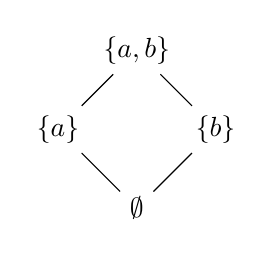
\begin{tikzpicture}[scale=1.0, auto]
  % Nodes
  \node (top) at (0,0) {$\{a,b\}$};
  \node (left) at (-1,-1) {$\{a\}$};
  \node (right) at (1,-1) {$\{b\}$};
  \node (bottom) at (0,-2) {$\emptyset$};

  % Edges
  \draw (left) -- (top);
  \draw (right) -- (top);
  \draw (bottom) -- (left);
  \draw (bottom) -- (right);
\end{tikzpicture}
\end{center}

\begin{theorem}
    Let $f \colon A \to B$ and $g \colon B \to C$ be functions. Suppose $g \circ f$ is onto (surjective) and $g$ is one-to-one (injective). Then $f$ is onto.
    \end{theorem}
    
    \begin{proof}
    \textbf{Step 1: Set up the problem.}\\
    We want to show that for every element $b \in B$, there exists an element $a \in A$ such that $f(a) = b$. 
    This is precisely the condition that $f$ is onto.
    
    \textbf{Step 2: Use that $g \circ f$ is onto.}\\
    Since $g \circ f$ is onto (surjective), for any element $c \in C$, there exists $a \in A$ such that
    \[
    (g \circ f)(a) = g(f(a)) = c.
    \]
    
    \textbf{Step 3: Relate $c$ to an arbitrary $b \in B$.}\\
    Fix any $b \in B$. Let $c = g(b)$. By onto-ness of $g \circ f$, there must be some $a \in A$ for which
    \[
    g\bigl(f(a)\bigr) = c = g(b).
    \]
    
    \textbf{Step 4: Use that $g$ is one-to-one.}\\
    Since $g$ is injective, the equality $g\bigl(f(a)\bigr) = g(b)$ implies
    \[
    f(a) = b.
    \]
    
    \textbf{Step 5: Conclude that $f$ is onto.}\\
    We have shown that for an arbitrary $b \in B$, we can find $a \in A$ with $f(a) = b$. Hence,
    \[
    \forall b \in B, \;\exists a \in A : f(a) = b,
    \]
    which is exactly the definition of $f$ being onto. This completes the proof.
    \end{proof}
\end{document}
